\documentclass[a4paper,12pt]{article}
\usepackage[utf8]{inputenc}
\usepackage[italian]{babel}
\usepackage[margin=2.5cm]{geometry}
\usepackage{graphicx}
\usepackage{amsmath,amssymb}
\usepackage{booktabs}
\usepackage{float}
\usepackage{caption}
\usepackage{hyperref}
\usepackage{setspace}
\onehalfspacing

\title{\textbf{Valore e Rischio di Portafoglio} \\ \large Analisi di 7 titoli azionari US e portafoglio equity}
\author{Francesco Mazzini}
\date{A.A.\ 2025--2026}

\begin{document}
\maketitle
\tableofcontents
\newpage

%==========================================================================
\section{Selezione titoli e rendimenti (Punto 1)}

Sono stati selezionati 7 titoli azionari quotati su mercati statunitensi dal dataset Bloomberg fornito. I titoli, tutti denominati in USD, sono:

\begin{table}[H]
\centering
\begin{tabular}{llcc}
\toprule
\# & Ticker Bloomberg & Settore & Peso portafoglio \\
\midrule
1 & DHR US Equity & Healthcare/Industrial & 10\% \\
2 & EW UN Equity & Medical Devices & 20\% \\
3 & HIG US Equity & Insurance & 10\% \\
4 & NDAQ US Equity & Financial Services & 10\% \\
5 & PANW US Equity & Cybersecurity & 10\% \\
6 & TDY US Equity & Aerospace/Defense & 10\% \\
7 & VRTX US Equity & Biotech/Pharma & 20\% \\
\bottomrule
\end{tabular}
\caption{Titoli selezionati con relativo peso nel portafoglio del Punto~4.}
\end{table}

Il campione copre il periodo dal 19 luglio 2021 al 17 novembre 2025 (1131 osservazioni giornaliere di prezzo, 1130 rendimenti).

I rendimenti sono calcolati come \textbf{log-rendimenti} giornalieri:
\[
g_t = \ln\!\left(\frac{P_t}{P_{t-1}}\right)
\]

In Figura~\ref{fig:prezzi} si riporta l'evoluzione dei prezzi normalizzati (base 100 alla prima data), che permette di confrontare le performance relative. In Figura~\ref{fig:rendimenti_log} sono mostrati i rendimenti log giornalieri per ciascun titolo.

\begin{figure}[H]
\centering
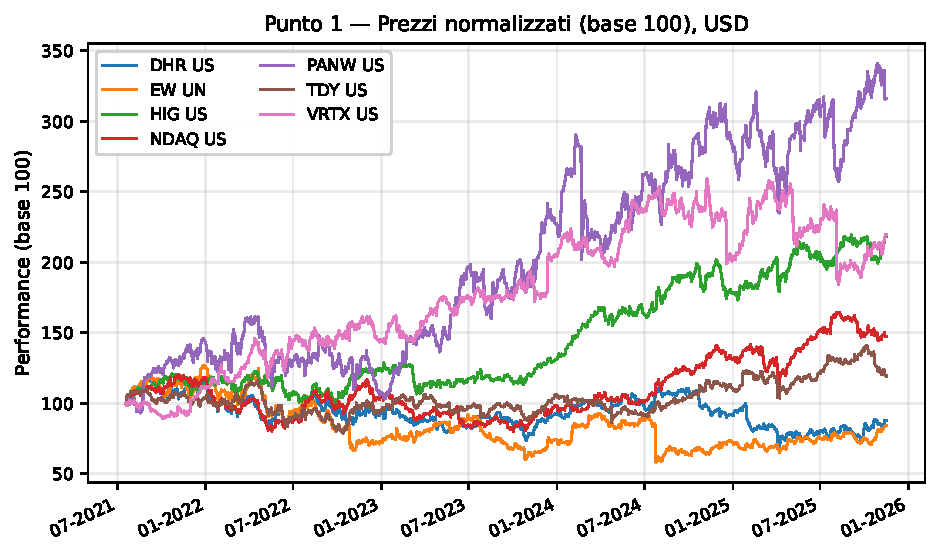
\includegraphics[width=\textwidth]{figures/p1_prezzi_normalizzati.pdf}
\caption{Prezzi normalizzati (base 100) dei 7 titoli selezionati.}
\label{fig:prezzi}
\end{figure}

\begin{figure}[H]
\centering
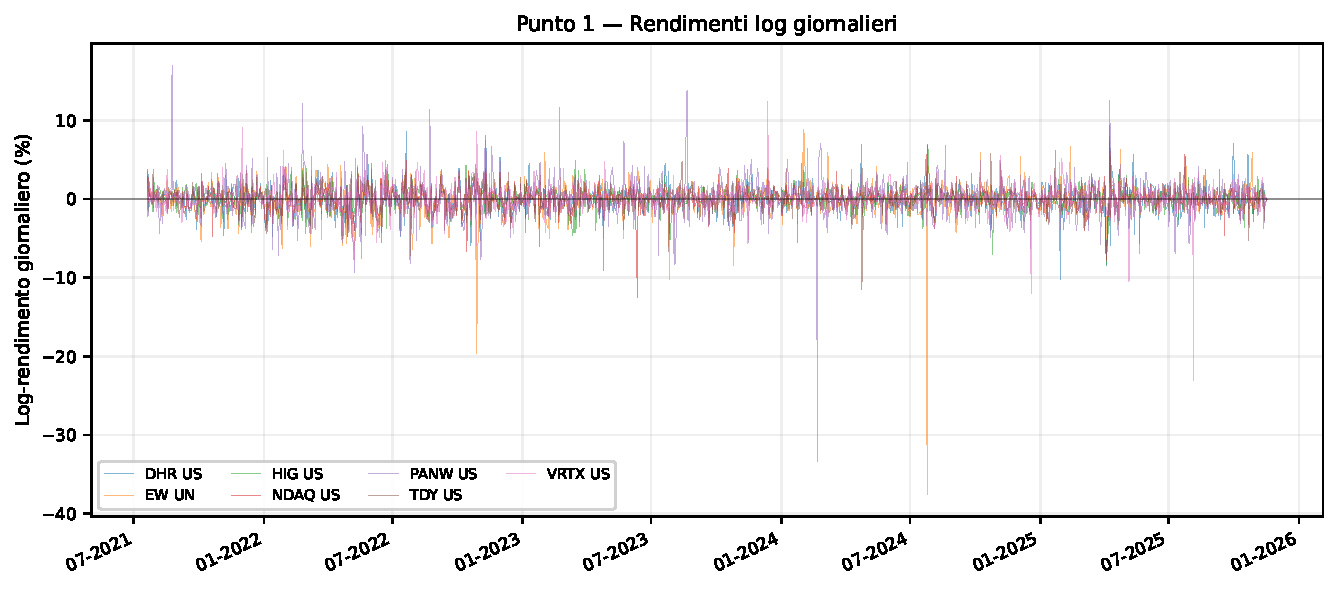
\includegraphics[width=\textwidth]{figures/p1_rendimenti_log.pdf}
\caption{Rendimenti log giornalieri (\%) per ciascun titolo.}
\label{fig:rendimenti_log}
\end{figure}

Si nota una forte eterogeneità nelle performance: PANW US ha quasi triplicato il suo valore (+216\%), mentre DHR US e EW UN hanno registrato rendimenti negativi nel periodo ($-12\%$ e $-16\%$ rispettivamente). HIG US e VRTX US hanno più che raddoppiato (+118\% e +119\%).


%==========================================================================
\section{Statistiche di sintesi, volatilità e correlazioni (Punto 2)}

\subsection{Statistiche descrittive}

Per ogni titolo si calcolano rendimento totale semplice, CAGR (tasso annuo composto), volatilità giornaliera e annualizzata, asimmetria e curtosi in eccesso.

\begin{table}[H]
\centering
\footnotesize
\begin{tabular}{lrrrrr}
\toprule
Titolo & Rend.\ totale & CAGR & $\sigma_{\text{ann}}$ & Skewness & Kurt.\ ecc. \\
\midrule
DHR US   & $-12.0\%$ & $-2.9\%$ & 27.7\% & 0.02 & 4.45 \\
EW UN    & $-16.1\%$ & $-4.0\%$ & 34.6\% & $-5.21$ & 84.1 \\
HIG US   & $+118.1\%$ & $+19.7\%$ & 21.9\% & $-0.39$ & 3.31 \\
NDAQ US  & $+47.5\%$ & $+9.4\%$ & 23.2\% & $-0.75$ & 7.65 \\
PANW US  & $+216.2\%$ & $+30.4\%$ & 41.4\% & $-1.40$ & 27.7 \\
TDY US   & $+19.3\%$ & $+4.2\%$ & 23.5\% & $-0.62$ & 6.21 \\
VRTX US  & $+119.4\%$ & $+19.9\%$ & 28.4\% & $-2.07$ & 30.7 \\
\bottomrule
\end{tabular}
\caption{Statistiche di sintesi sui log-rendimenti giornalieri.}
\label{tab:summary}
\end{table}

Il test di Jarque-Bera rifiuta l'ipotesi di normalità per tutti i titoli ($p < 10^{-100}$), confermando la presenza di code pesanti e asimmetria negativa tipiche dei rendimenti azionari. In particolare, EW UN presenta un eccesso di curtosi estremo (84.1) dovuto a un outlier di $-37.6\%$ il 25 luglio 2024.

\begin{figure}[H]
\centering
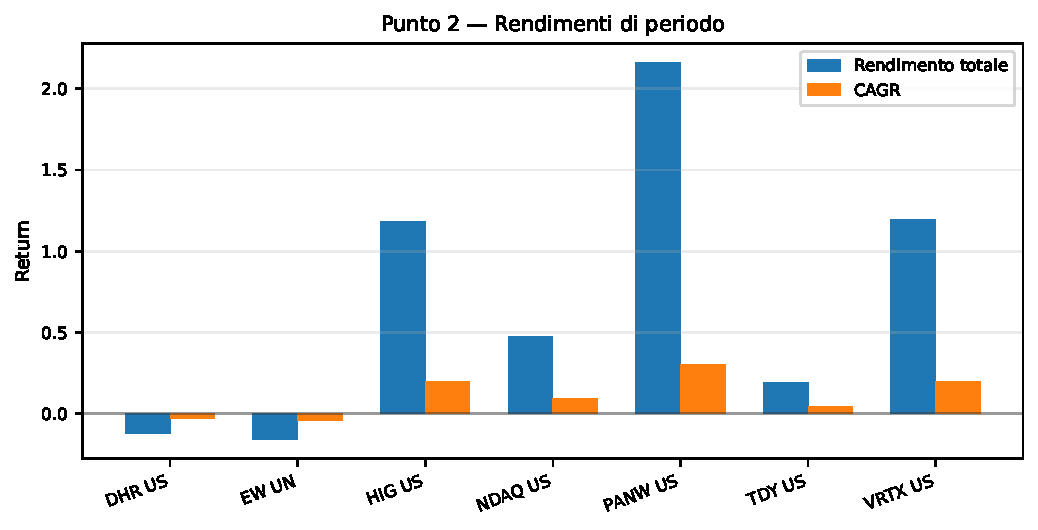
\includegraphics[width=0.95\textwidth]{figures/p2_rendimenti.pdf}
\caption{Rendimenti totali e CAGR per titolo.}
\end{figure}

\subsection{Volatilità su diverse finestre}

La volatilità è calcolata come deviazione standard dei log-rendimenti giornalieri, annualizzata con il fattore $\sqrt{252}$ (giorni di trading/anno). Si utilizzano tre approcci:

\begin{itemize}
\item \textbf{Rolling}: media mobile della deviazione standard su finestre di 21 giorni ($\approx$1 mese), 63 giorni ($\approx$3 mesi) e 252 giorni ($\approx$1 anno).
\item \textbf{EWMA RiskMetrics}: media mobile esponenziale con $\lambda = 0.94$ e inizializzazione su 30 giorni:
\[
\sigma^2_t = \lambda\,\sigma^2_{t-1} + (1-\lambda)\,r^2_{t-1}
\]
\item \textbf{GARCH(1,1)-Student-$t$}: modello a volatilità condizionata stimato via MLE, con distribuzione delle innovazioni a code pesanti (Student-$t$). Se la stima GARCH converge a una soluzione di frontiera ($\hat\beta \leq 10^{-4}$), si utilizza come fallback EGARCH(1,1,1)-$t$, poi GARCH-Normale, poi EGARCH-Normale.
\end{itemize}

\begin{figure}[H]
\centering
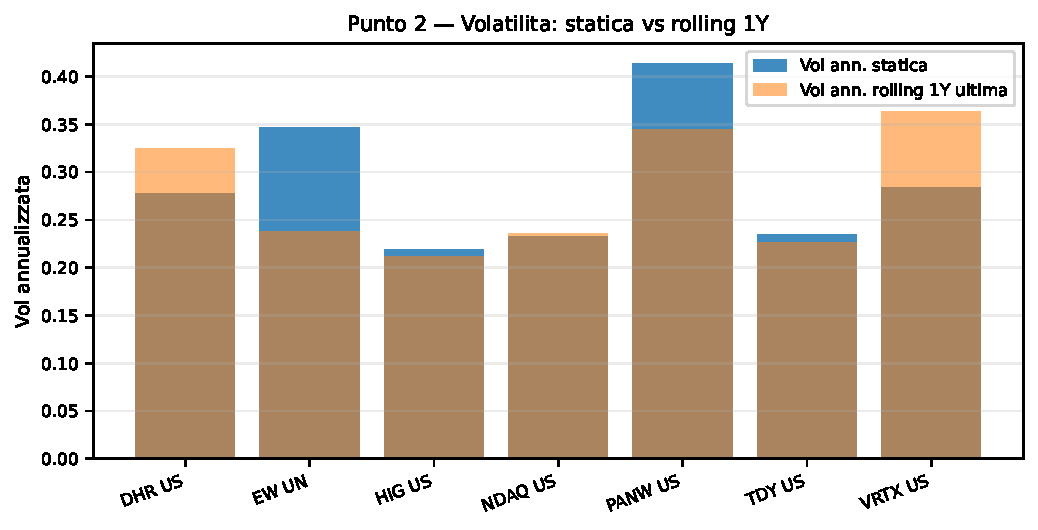
\includegraphics[width=0.95\textwidth]{figures/p2_vol_statica_vs_roll1y.pdf}
\caption{Volatilità annualizzata: statica (intero campione) vs rolling 1 anno (ultima osservazione).}
\end{figure}

\begin{figure}[H]
\centering
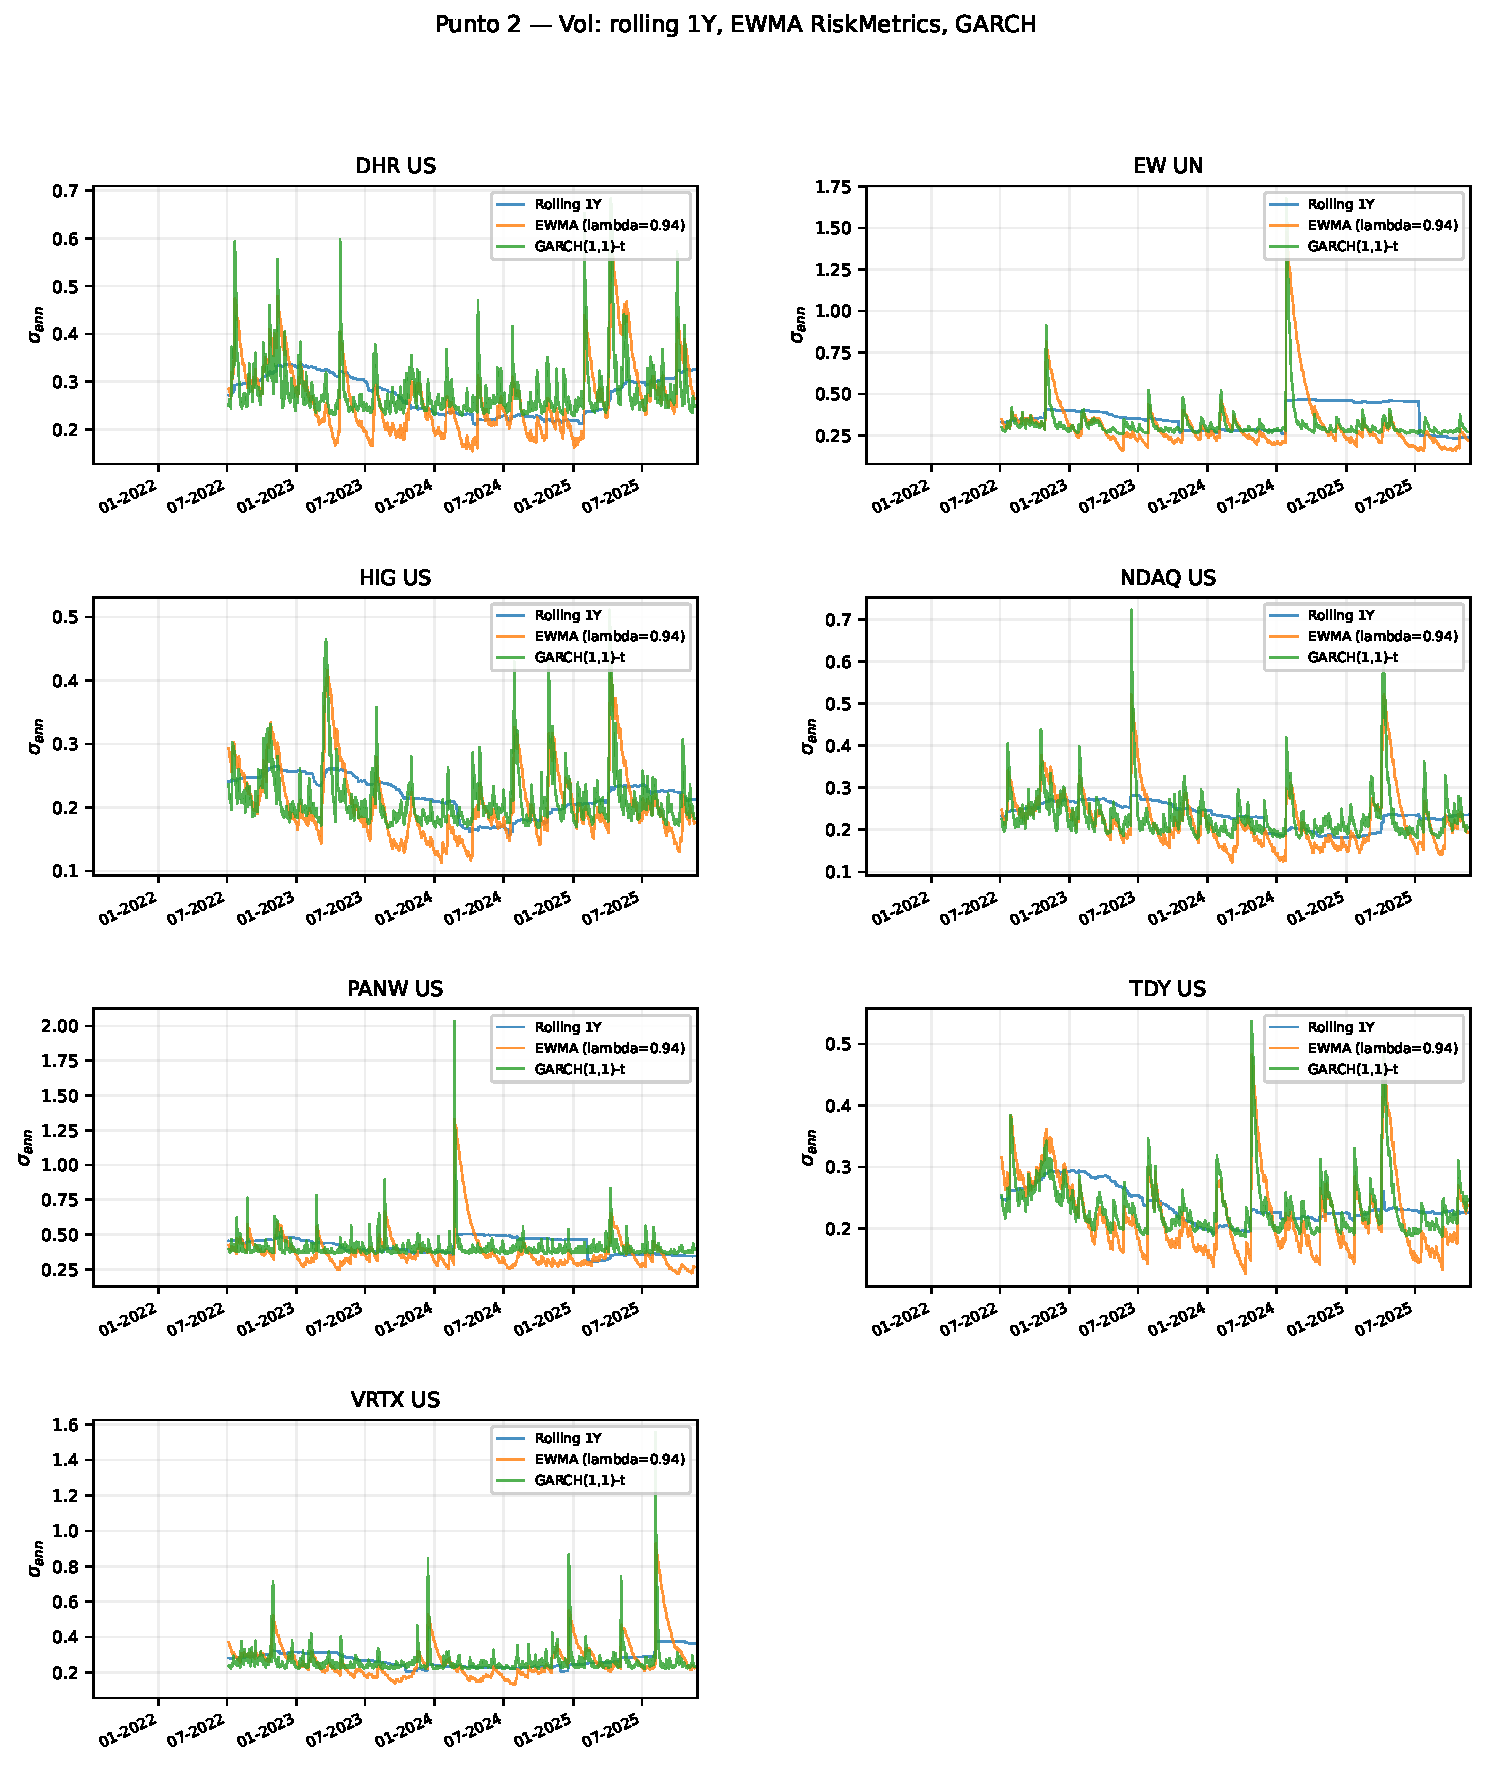
\includegraphics[width=\textwidth]{figures/p2_vol_pannelli.pdf}
\caption{Confronto vol.\ rolling 1Y, EWMA RiskMetrics e GARCH per ciascun titolo.}
\label{fig:vol_pannelli}
\end{figure}

La Figura~\ref{fig:vol_pannelli} mostra che la volatilità non è costante nel tempo: tutti i titoli presentano cluster di alta volatilità (volatility clustering), ben catturati dai modelli EWMA e GARCH.

\subsection{Matrice di correlazione e test di significatività}

La matrice di correlazione di Pearson è stimata sui log-rendimenti in campione listwise ($n = 1130$). Per ogni coppia $(i,j)$ si testa $H_0: \rho_{ij} = 0$ contro l'alternativa bilaterale, con la statistica:
\[
t_{ij} = \hat\rho_{ij}\sqrt{\frac{n-2}{1-\hat\rho_{ij}^2}} \;\sim\; t_{n-2}
\]

Al livello $\alpha = 5\%$ (due code), tutte le 21 coppie risultano significativamente diverse da zero. Le correlazioni sono tutte positive, con media $|\hat\rho| = 0.29$, massimo $\hat\rho = 0.46$ (NDAQ--TDY) e minimo $\hat\rho = 0.14$ (EW--VRTX).

\begin{figure}[H]
\centering
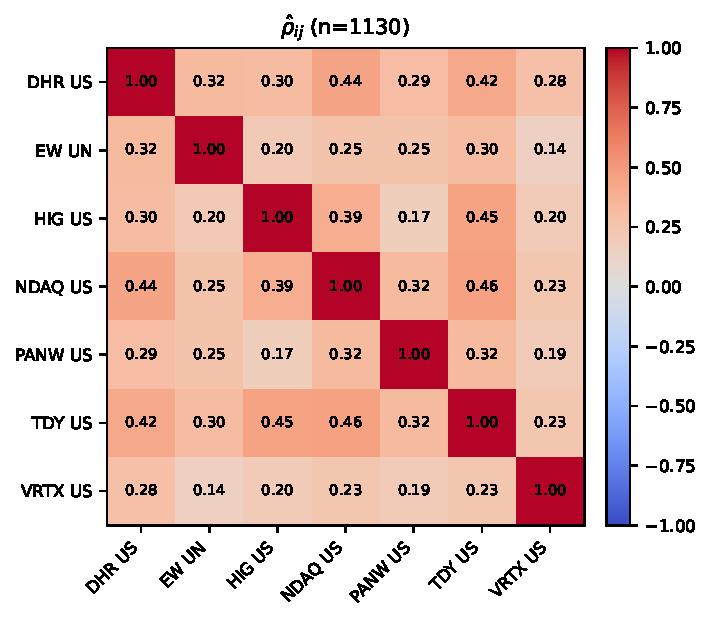
\includegraphics[width=0.55\textwidth]{figures/p2_heatmap_rho.pdf}
\caption{Heatmap delle correlazioni di Pearson.}
\end{figure}

\begin{figure}[H]
\centering
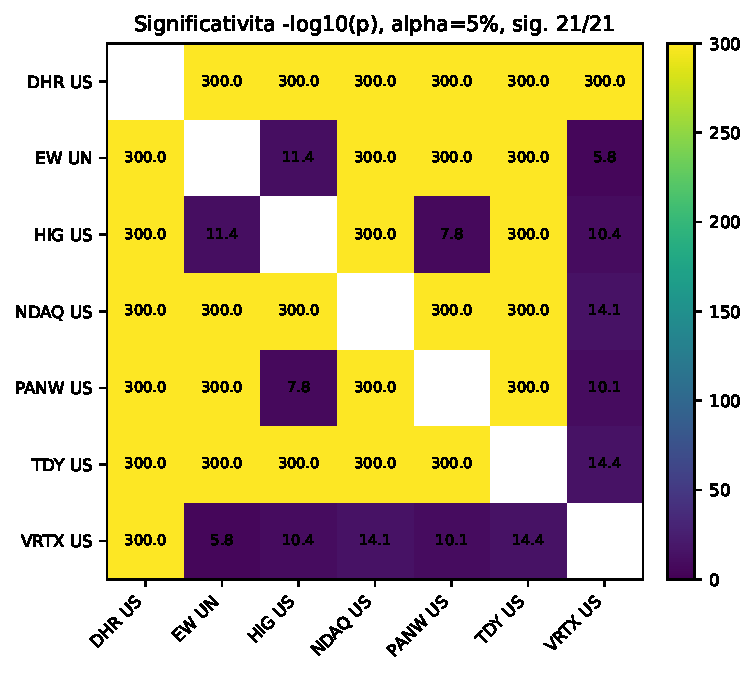
\includegraphics[width=0.6\textwidth]{figures/p2_heatmap_pval.pdf}
\caption{Significatività statistica: $-\log_{10}(p)$. Valori più alti indicano maggiore significatività.}
\end{figure}


%==========================================================================
\section{Value-at-Risk per singolo titolo (Punto 3)}

Il VaR è stimato al livello $\alpha = 5\%$ (coda sinistra) con orizzonte $H = 1$ giorno sui log-rendimenti giornalieri. Il VaR è riportato come magnitudine positiva di perdita: $\text{VaR}_g = -Q_\alpha(g)$. Per la conversione in USD su una posizione long di $N = 100\,000$ \$:
\[
\text{VaR}_{\text{USD}} = N\left(1 - e^{-\text{VaR}_g}\right)
\]

Vengono utilizzati tre metodi.

\subsection{VaR parametrico gaussiano}

Si assume $g_t \sim N(\hat\mu, \hat\sigma^2)$ con $\hat\mu$ e $\hat\sigma$ stimati dal campione:
\[
\text{VaR}_g = -\left(\hat\mu + z_\alpha\,\hat\sigma\right), \qquad z_\alpha = \Phi^{-1}(\alpha) \approx -1.645
\]

\subsection{VaR storico}

Il quantile empirico al livello $\alpha$ sui rendimenti osservati: $\text{VaR}_g = -Q_\alpha^{\text{emp}}(g)$.

\subsection{VaR Monte Carlo via Moto Browniano Geometrico}

La simulazione è basata sul \textbf{Moto Browniano Geometrico} (GBM). Il prezzo segue:
\[
\frac{dS}{S} = \mu\,dt + \sigma\,dW
\]
da cui il log-rendimento discretizzato su un giorno ($dt = 1/252$ anni):
\[
g_t = \left(\mu_{\text{ann}} - \frac{\sigma_{\text{ann}}^2}{2}\right)dt + \sigma_{\text{ann}}\sqrt{dt}\;Z, \qquad Z \sim N(0,1)
\]

I parametri annualizzati sono stimati dai dati giornalieri:
\begin{align}
\hat\sigma_{\text{ann}} &= \hat\sigma_{\text{gg}} \cdot \sqrt{252} \\
\hat\mu_{\text{ann}} &= \hat\mu_{\text{gg}} \cdot 252 + \frac{\hat\sigma_{\text{ann}}^2}{2}
\end{align}
dove $\hat\mu_{\text{gg}}$ è la media campionaria dei log-rendimenti e $\hat\sigma_{\text{gg}}$ la deviazione standard campionaria.

Il drift giornaliero del log-rendimento è $(\hat\mu_{\text{ann}} - \hat\sigma_{\text{ann}}^2/2) \cdot dt = \hat\mu_{\text{gg}}$ e la componente stocastica è $\hat\sigma_{\text{ann}} \sqrt{dt} = \hat\sigma_{\text{gg}}$.

Si generano $N = 50\,000$ simulazioni indipendenti. Il VaR è il quantile empirico al livello $\alpha$ dei rendimenti simulati.

\begin{table}[H]
\centering
\begin{tabular}{lrrr}
\toprule
Titolo & VaR param.\ (USD) & VaR storico (USD) & VaR MC GBM (USD) \\
\midrule
DHR US   & 2\,844 & 2\,679 & 2\,851 \\
EW UN    & 3\,540 & 2\,694 & 3\,530 \\
HIG US   & 2\,172 & 2\,175 & 2\,178 \\
NDAQ US  & 2\,345 & 2\,267 & 2\,333 \\
PANW US  & 4\,100 & 3\,727 & 4\,088 \\
TDY US   & 2\,389 & 2\,285 & 2\,403 \\
VRTX US  & 2\,830 & 2\,326 & 2\,818 \\
\bottomrule
\end{tabular}
\caption{VaR a 1 giorno, $\alpha = 5\%$, su posizione long di 100\,000 USD per titolo.}
\label{tab:var}
\end{table}

Il VaR parametrico e il MC GBM producono risultati molto simili (differenza $<1\%$), come atteso dato che condividono l'ipotesi gaussiana. Lo storico è generalmente più basso, tranne per HIG US dove i tre metodi sono quasi allineati.

\subsection{Backtest out-of-sample}

Il campione è diviso a metà: il VaR è stimato sulla prima parte (50\%) e le violazioni sono contate sulla seconda. Con $\alpha = 5\%$, ci si attende circa il 5\% di violazioni. I risultati mostrano che per la maggior parte dei titoli le violazioni sono inferiori al 5\%, indicando stime conservative.

\begin{figure}[H]
\centering
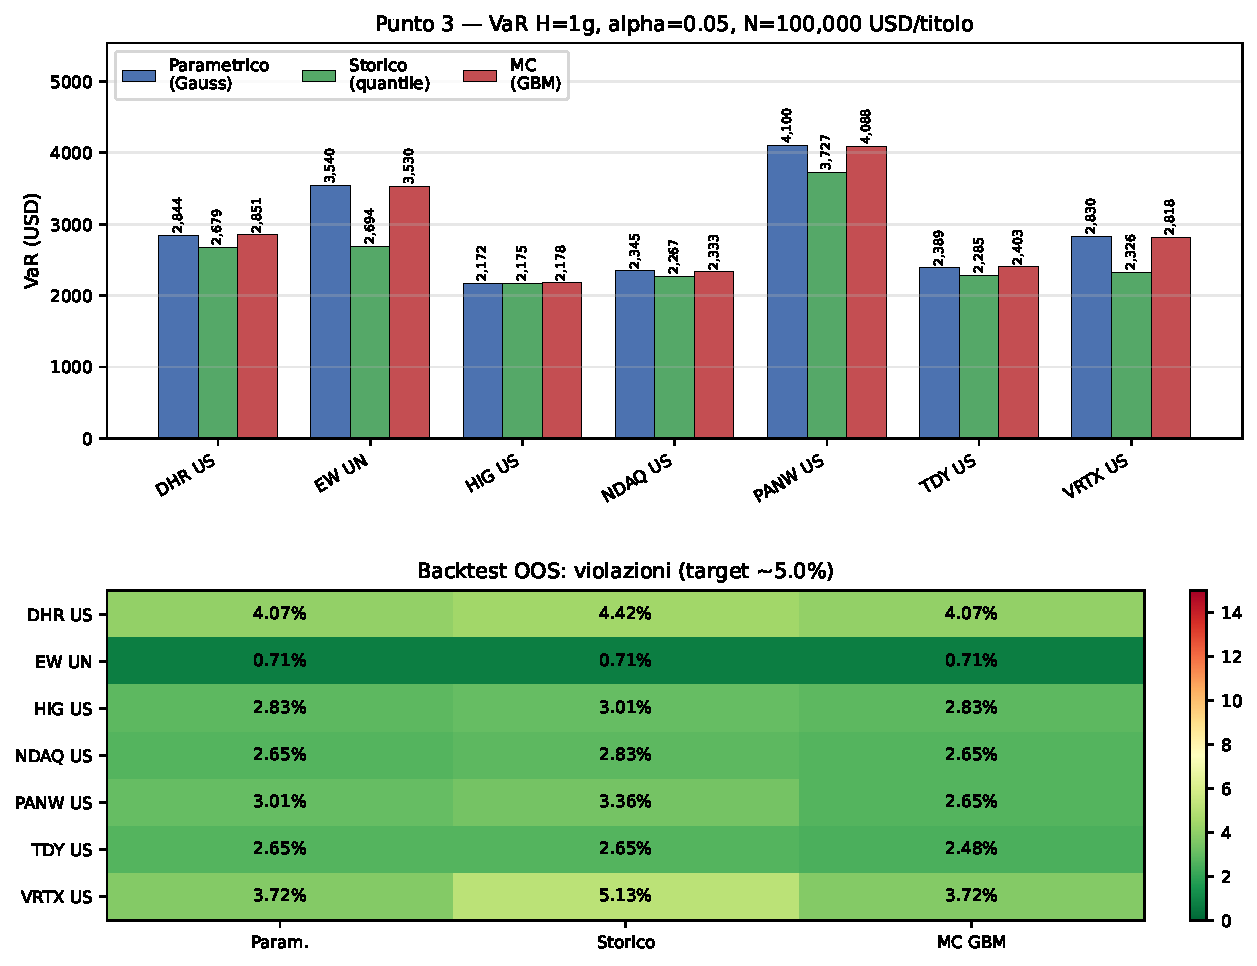
\includegraphics[width=\textwidth]{figures/p3_var_e_violazioni.pdf}
\caption{VaR per titolo (USD) e backtest OOS: percentuale di violazioni.}
\label{fig:var}
\end{figure}


%==========================================================================
\section{Analisi del portafoglio (Punto 4)}

\subsection{Valore del portafoglio a pesi costanti (4.a)}

Si considera un investimento iniziale di $N = 100\,000$ USD, allocato secondo i pesi della consegna (Tabella~1), con il 10\% in liquidità (rendimento nullo, volatilità zero, correlazione zero con gli altri componenti). La strategia è \textbf{buy-and-hold} (pesi costanti, senza ribilanciamento giornaliero):
\[
V(t) = N\left(\sum_{i=1}^{7} w_i \frac{P_i(t)}{P_i(t_0)} + w_{\text{cash}}\right)
\]

La finestra è di 3 anni (dal 17 novembre 2022 al 17 novembre 2025, 783 osservazioni).

\begin{figure}[H]
\centering
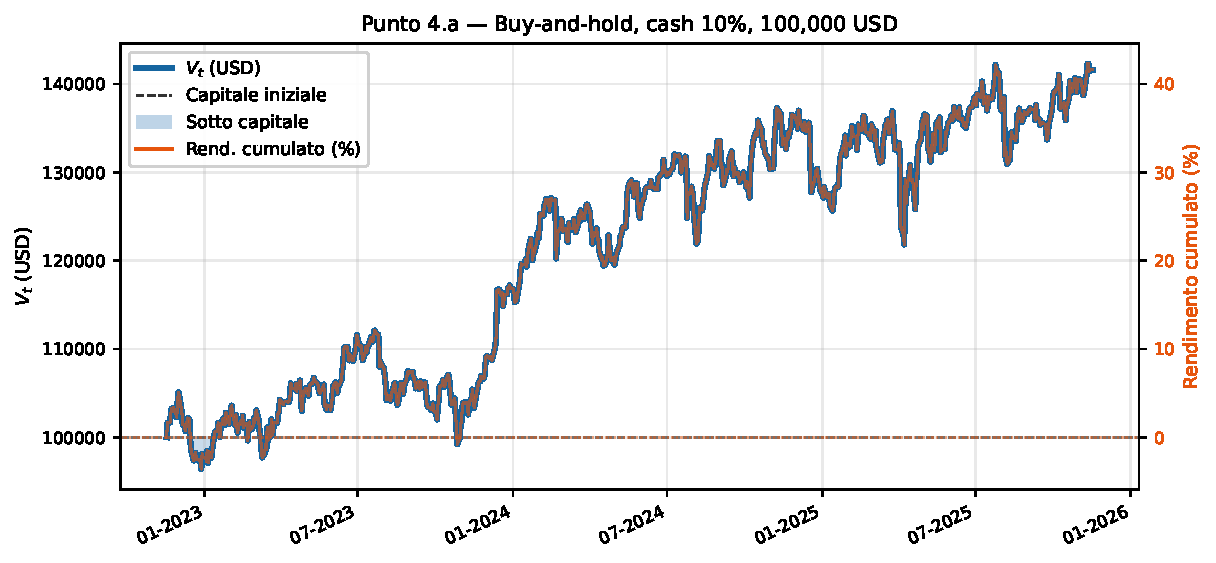
\includegraphics[width=\textwidth]{figures/p4a_portafoglio.pdf}
\caption{Evoluzione del valore del portafoglio e rendimento cumulato.}
\end{figure}

Il portafoglio raggiunge un valore finale di circa 141\,580 USD, con un rendimento complessivo del $+41.6\%$ (log: $+34.8\%$) in 3 anni.

\subsection{Rendimenti e volatilità del portafoglio (4.b)}

I rendimenti giornalieri del portafoglio sono calcolati come $g_{p,t} = \ln(V_t / V_{t-1})$. La volatilità rolling è stimata su finestre di 21 giorni (1 mese) e annualizzata con $\sqrt{252}$.

\begin{itemize}
\item Rendimento log totale: $+34.8\%$
\item Volatilità giornaliera campionaria: 0.96\%
\item Volatilità annualizzata: 15.2\%
\end{itemize}

\begin{figure}[H]
\centering
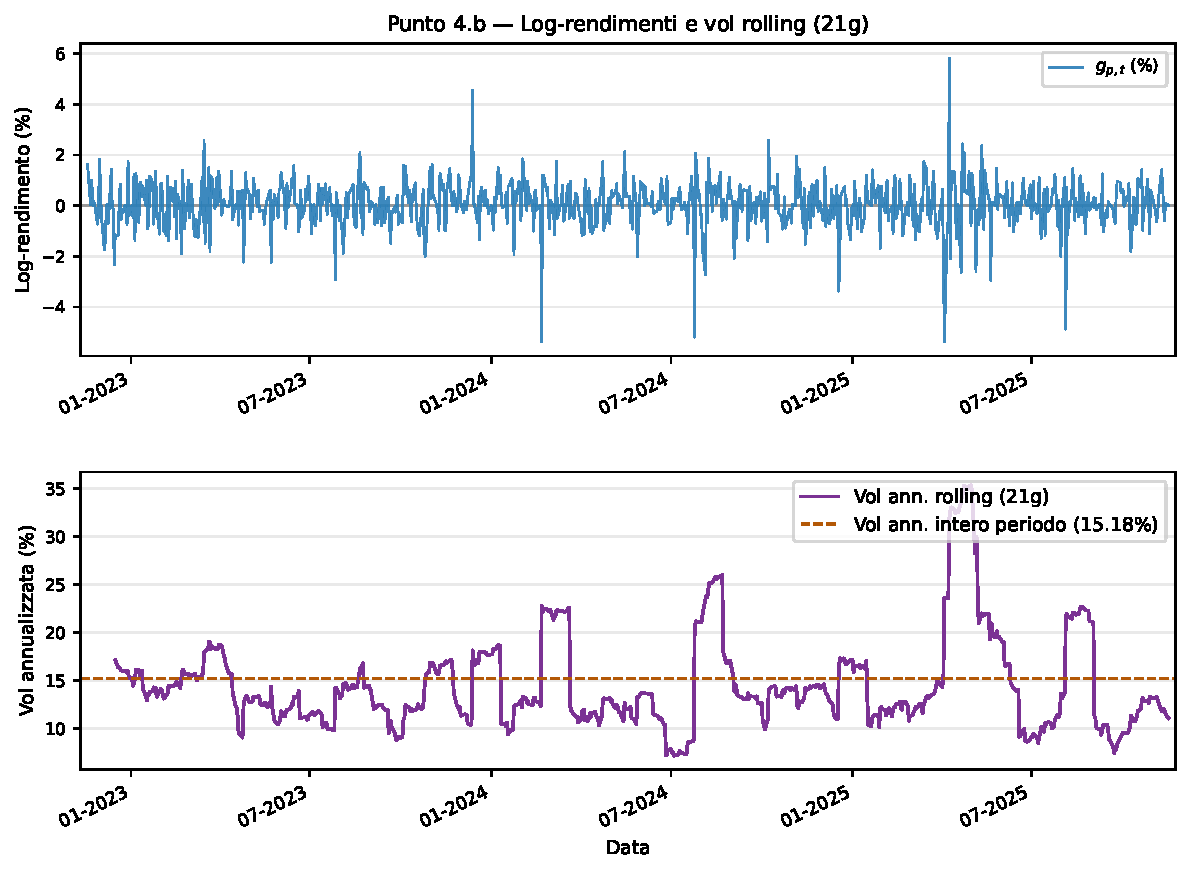
\includegraphics[width=\textwidth]{figures/p4b_rendimenti_vol.pdf}
\caption{Log-rendimenti giornalieri e volatilità rolling annualizzata del portafoglio.}
\end{figure}

\subsection{VaR del portafoglio (4.c)}

Il VaR del portafoglio è stimato con tre metodi:

\paragraph{Parametrico (varianza-covarianza).} Si stima la matrice di covarianza $\hat\Sigma$ sui log-rendimenti azionari nella finestra di 3 anni ($n = 783$). La liquidità non compare in $\hat\Sigma$ (vol = 0). Il rendimento e la volatilità del portafoglio sono:
\[
\hat\mu_p = \mathbf{w}'\hat{\boldsymbol\mu}, \qquad \hat\sigma_p = \sqrt{\mathbf{w}'\hat\Sigma\,\mathbf{w}}
\]
dove $\mathbf{w}$ sono i pesi azionari (che sommano al 90\%). Il VaR gaussiano è $\text{VaR}_g = -(\hat\mu_p + z_\alpha\hat\sigma_p)$.

\paragraph{Monte Carlo GBM multivariato (Cholesky).} Ogni titolo segue un GBM con moti browniani correlati. Si fattorizza la matrice di correlazione $\hat R$ via Cholesky ($\hat R = LL'$), poi:
\begin{enumerate}
\item Si generano $Z \sim N(\mathbf{0}, I_7)$ (shock indipendenti)
\item Si calcolano $\varepsilon = Z \cdot L'$ (shock correlati)
\item Il log-rendimento di ogni titolo è $g_i = \text{drift}_i + \text{vol}_i \cdot \varepsilon_i$
\item Il rendimento del portafoglio è $g_p = \sum_i w_i \cdot g_i$
\end{enumerate}
Si ripete per $N = 50\,000$ simulazioni e si prende il quantile al 5\%.

\paragraph{Storico.} Quantile empirico su $g_{p,t} = \ln(V_t/V_{t-1})$ del portafoglio 4.a.

\begin{table}[H]
\centering
\begin{tabular}{lcc}
\toprule
Metodo & VaR$_g$ (log-rend.) & VaR (USD) \\
\midrule
Parametrico (var-cov) & 0.01478 & 1\,467 \\
MC GBM (Cholesky) & 0.01472 & 1\,461 \\
Storico su $g_p$ & 0.01347 & 1\,338 \\
\bottomrule
\end{tabular}
\caption{VaR portafoglio a 1 giorno, $\alpha = 5\%$, capitale 100\,000 USD.}
\end{table}

Il parametrico e il MC GBM differiscono dello 0.4\%, confermando la coerenza delle stime (la differenza è rumore di campionamento Monte Carlo). Lo storico è leggermente inferiore ($-8.8\%$), coerente con il fatto che la distribuzione empirica dei rendimenti del portafoglio non presenta code particolarmente pesanti nel periodo analizzato.

\begin{figure}[H]
\centering
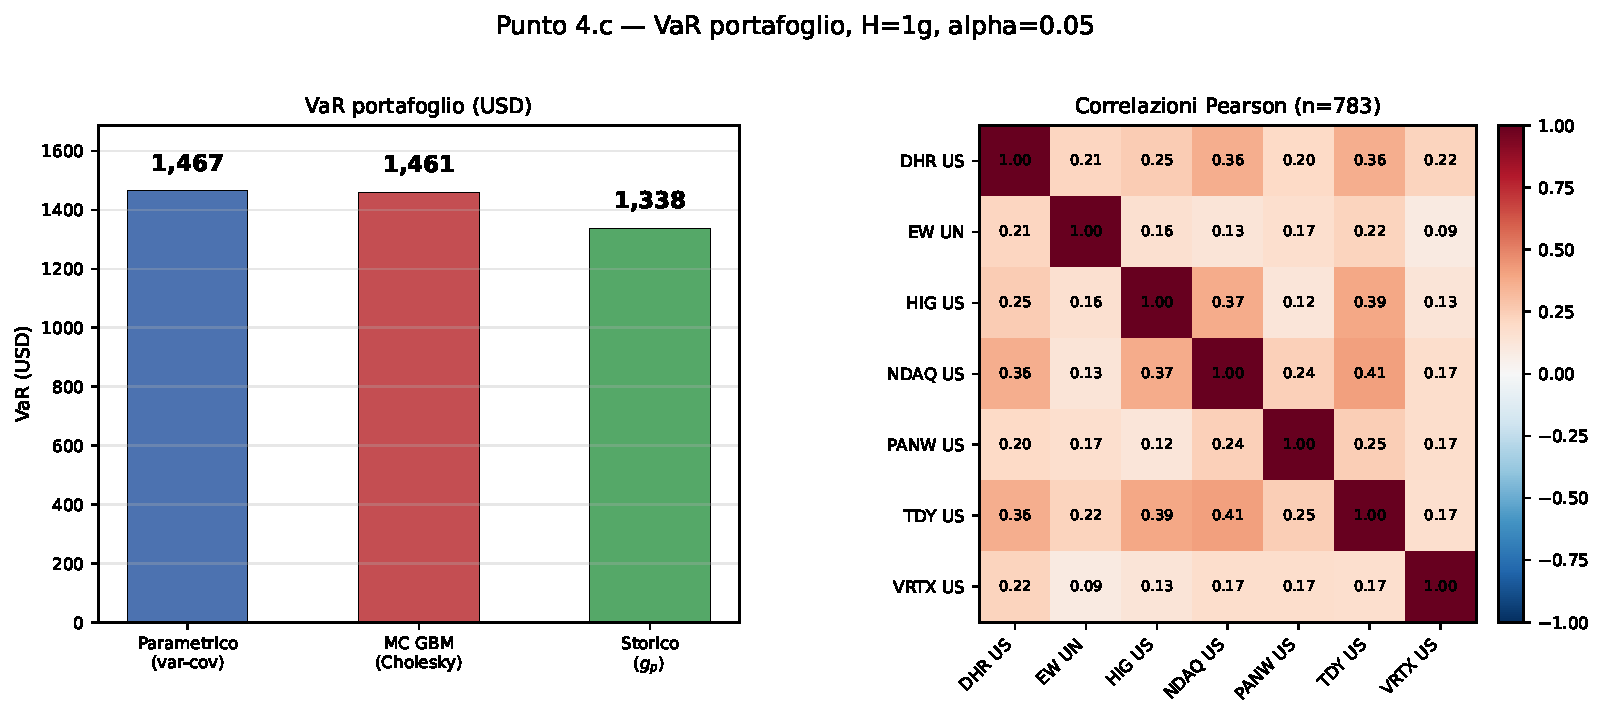
\includegraphics[width=\textwidth]{figures/p4c_var_ptf.pdf}
\caption{VaR del portafoglio (USD) e matrice di correlazione Pearson usata nel parametrico.}
\end{figure}

\subsection{Diversificazione e correlazioni (4.d)}

Per valutare il beneficio della diversificazione, si confronta il VaR parametrico con la matrice $\hat\Sigma$ completa e con la matrice diagonale (stesse volatilità marginali, correlazioni nulle):

\begin{itemize}
\item $\hat\sigma_p$ con $\hat\Sigma$ completa: 0.92\% giornaliera
\item $\hat\sigma_p$ con $\hat\Sigma$ diagonale ($\rho = 0$): 0.67\% giornaliera
\item \textbf{Diversification ratio} $= 1 - \sigma_p / \sum_i w_i\sigma_i = 0.424$
\end{itemize}

Il rapporto di diversificazione del 42.4\% indica che la volatilità del portafoglio è significativamente inferiore a quella del caso peggiore (correlazione perfetta tra tutti i titoli), segno di un beneficio tangibile dalla diversificazione.

Tuttavia, poiché le correlazioni sono tutte positive (media $|\hat\rho| = 0.23$), il VaR con la matrice completa è \textbf{superiore} a quello con asset indipendenti: 1\,467 USD contro 1\,057 USD (+410 USD, $+38.7\%$). Questo è atteso: correlazioni positive aumentano la varianza del portafoglio rispetto al caso di indipendenza.

Il VaR storico (1\,338 USD) è inferiore al parametrico su questo campione, suggerendo che la distribuzione empirica dei rendimenti del portafoglio non presenta code particolarmente pesanti.

\begin{figure}[H]
\centering
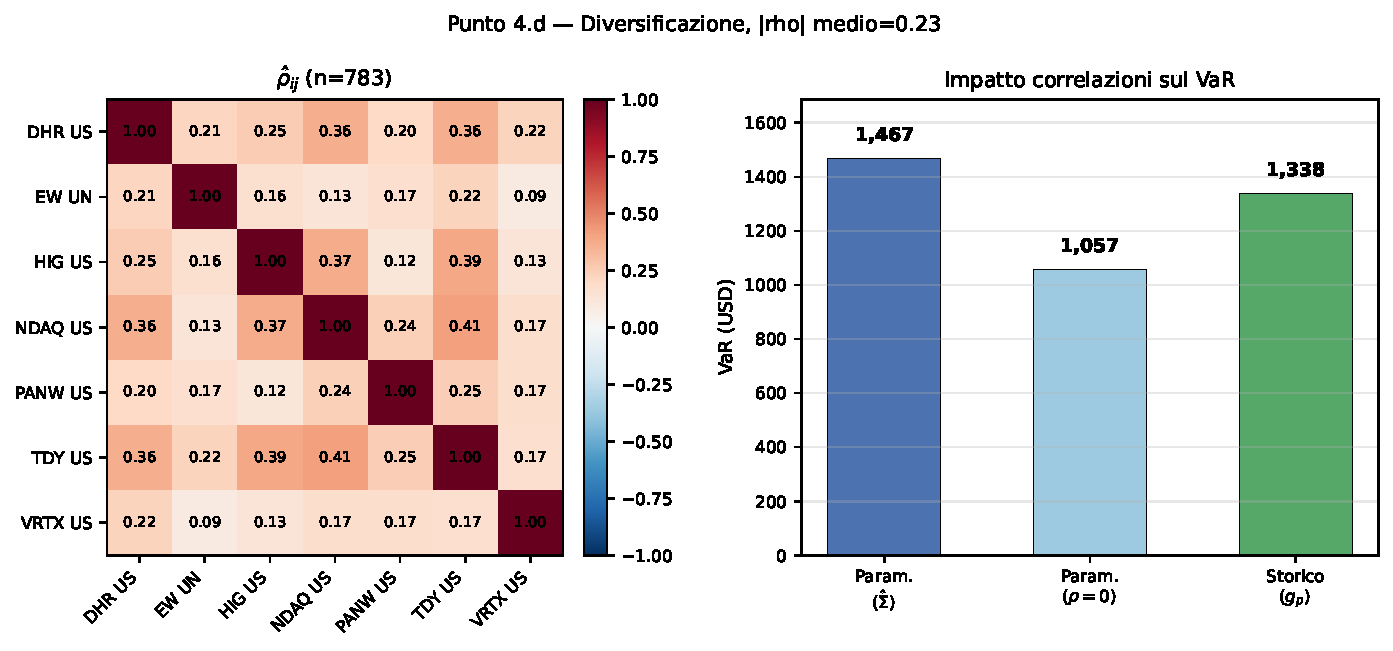
\includegraphics[width=\textwidth]{figures/p4d_diversificazione.pdf}
\caption{Impatto delle correlazioni sul VaR e matrice di correlazione.}
\end{figure}

\subsection{Dinamica della volatilità (4.e)}

Si analizza se la volatilità del portafoglio appare costante o presenta dinamiche significative nei 3 anni considerati. Si utilizzano diversi approcci:

\paragraph{Analisi grafica.} La volatilità rolling a 1 anno varia da un minimo del 13.4\% (dicembre 2023) a un massimo del 17.6\% (luglio 2025), con un rapporto max/min di 1.31. L'EWMA e il GARCH(1,1)-$t$ confermano la variabilità nel tempo.

\paragraph{Sotto-periodi.} Dividendo il campione in 3 parti uguali:

\begin{table}[H]
\centering
\begin{tabular}{lccc}
\toprule
Periodo & Date & $n$ & $\sigma_{\text{ann}}$ \\
\midrule
P1 & nov 2022 -- nov 2023 & 260 & 13.9\% \\
P2 & nov 2023 -- nov 2024 & 261 & 15.0\% \\
P3 & nov 2024 -- nov 2025 & 261 & 16.5\% \\
\bottomrule
\end{tabular}
\caption{Volatilità per sotto-periodo.}
\end{table}

\paragraph{Test statistici.}

\begin{table}[H]
\centering
\begin{tabular}{lcc}
\toprule
Test & Statistica & $p$-value \\
\midrule
Engle ARCH-LM (lag = 10) & 31.84 & $4.3 \times 10^{-4}$ \\
Ljung-Box su $g_p^2$ (lag = 20) & 36.93 & $1.2 \times 10^{-2}$ \\
Bartlett (3 sotto-periodi) & 7.52 & 0.023 \\
Levene (3 sotto-periodi) & 0.67 & 0.510 \\
\bottomrule
\end{tabular}
\caption{Test sulla dinamica della volatilità.}
\end{table}

Il test di Engle ARCH-LM rifiuta fortemente $H_0$ (assenza di eteroschedasticità condizionata) con $p = 4.3 \times 10^{-4}$, confermando la presenza di \textbf{volatility clustering}. Il Ljung-Box sui rendimenti al quadrato conferma ($p = 0.012$). Il test di Bartlett rifiuta l'uguaglianza delle varianze tra sotto-periodi ($p = 0.023$), mentre il test di Levene (robusto alla non-normalità) non rifiuta ($p = 0.51$), suggerendo che la differenza tra sotto-periodi non è estrema.

Il modello GARCH(1,1)-Student-$t$ stimato sul portafoglio ha persistenza $\hat\alpha_1 + \hat\beta_1 = 0.855$, indicando che gli shock di volatilità sono marcatamente persistenti.

\textbf{Conclusione}: la volatilità del portafoglio \emph{non appare costante}. Pur con variazioni moderate in ampiezza (ratio max/min = 1.31), l'evidenza statistica di eteroschedasticità condizionata è forte (ARCH-LM $p < 0.001$), e la persistenza GARCH conferma dinamiche significative nella volatilità.

\begin{figure}[H]
\centering
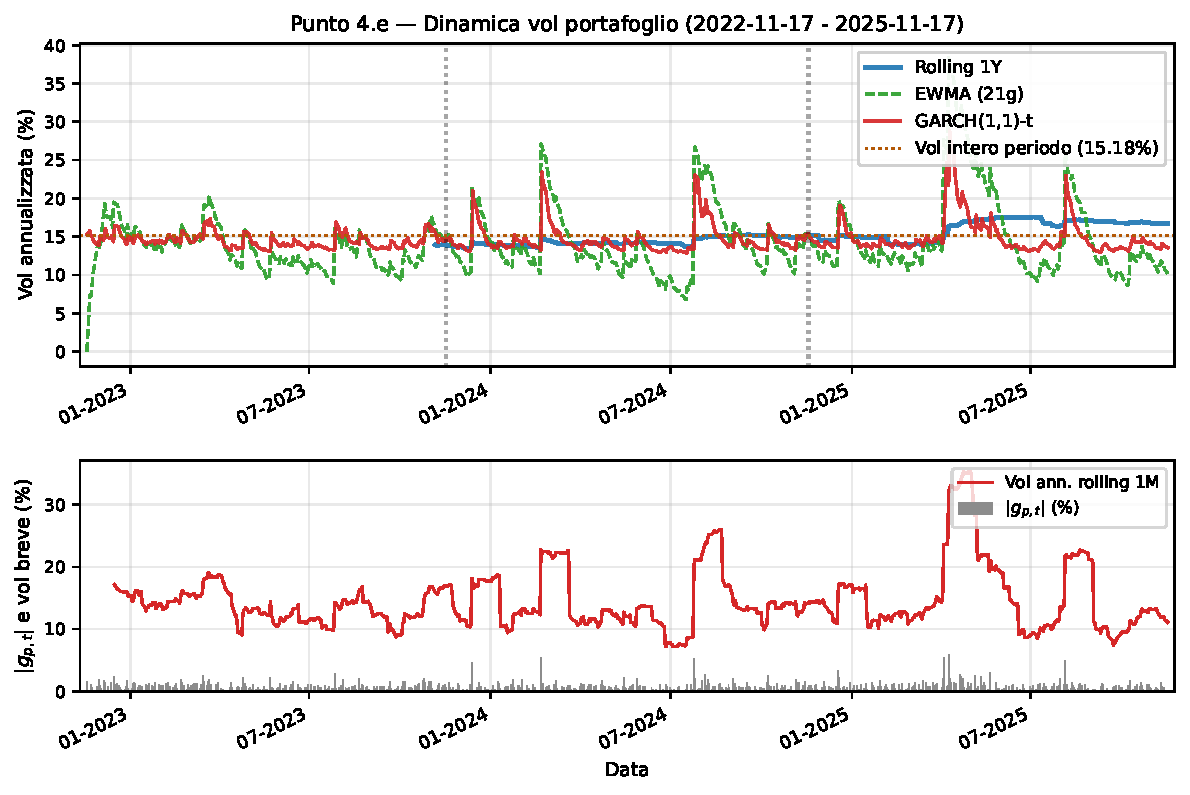
\includegraphics[width=\textwidth]{figures/p4e_vol_dinamica.pdf}
\caption{Dinamica della volatilità del portafoglio: stime rolling, EWMA, GARCH e $|g_{p,t}|$.}
\end{figure}


%==========================================================================
\section{Nota metodologica}

\begin{itemize}
\item I parametri $\alpha$ (livello di confidenza del VaR) e $H$ (orizzonte in giorni) sono definiti come variabili nella prima cella del notebook e utilizzati in tutte le formule, garantendo flessibilità del modello.
\item Il numero di simulazioni Monte Carlo ($N = 50\,000$) e il seed ($= 42$) sono anch'essi parametri modificabili.
\item I 252 giorni di trading annui sono usati per l'annualizzazione della volatilità.
\item La liquidità è trattata come asset a rendimento nullo, coerentemente con la consegna.
\end{itemize}

\end{document}
